\documentclass[12pt, a4 paper]{article}
\usepackage[T2A]{fontenc}
\usepackage[utf8]{inputenc}
\usepackage[russian,english]{babel}
\usepackage{amsmath,amssymb,amsfonts,amsthm}
\usepackage{indentfirst}
\usepackage{titlesec}
\usepackage{graphicx}
\usepackage{setspace}

\titleformat*{\section}{\Large\bfseries\filcenter}
\titleformat*{\subsection}{\large\bfseries\filcenter}
\titleformat*{\subsubsection}{\normalsize\bfseries\filcenter}

\usepackage{cmap}                   % поиск в PDF

\usepackage{geometry}
    \geometry{top=20mm}
    \geometry{bottom=20mm}
    \geometry{left=30mm}
    \geometry{right=15mm}		

\theoremstyle{plain}
\newtheorem{definition}{Определение}		

		
 
%======================================================================
%======================================================================


\begin{document}
\selectlanguage{russian}

\section*{Реферат}
\addcontentsline{toc}{section}{Реферат}

\pagestyle{empty} % нумерация выкл.

\newpage
%====================================================

\setstretch{1.5}

\tableofcontents

\newpage


%=======================================================================
\setcounter{page}{4}

\section*{Введение}
\addcontentsline{toc}{section}{Введение}
\pagestyle{plain} % нумерация вкл.

Самолёты крепко обосновались в нашей жизни. Уже в середине прошлого века самолёт не был чем-то необычным. А время шло. И вот уже миллионы людей летают ежемесячно по всему миру на самых разнообразных воздушных лайнерах.

Но самолёты не автомобили – они намного массивнее и много менее поворотливы. А самое главное отличие состоит в том, что во время полёта они не могут остановиться в случае опасности, когда для автомобиля это один из самых безопасных способов разрешить сложную ситуацию. Это всё не доставляло особых проблем, пока самолёты были явлением редким, экспериментальным. Но в связи с постоянно растущим авиапарком у компаний возникла потребность в регулировке движения этих мастодонтов. Поэтому оказались чрезвычайно важными грамотная и своевременная дача указаний к движению воздушных бортов. У человечества к тому времени был обширный опыт регулирования наземного и водного транспорта, поэтому для разработки новых правил движения широко использовался эти наработки. Но всё равно воздух это другая стихия. И помимо стандартных решений нужны были новые.

Если на трассе между городами всё было более-менее понятно и решения имеющихся проблем нашлись довольно быстро. А вот вблизи больших городов, когда в аэропорт прилетают самолёты отовсюду, надо было принимать серьёзные меры.

Самым первым, и использующимся по сей день, стало расписание полётов. Но расписание это разграничения в рамках часов, а когда к аэропорту подлетают самолёты для посадки, нужны решения с точностью до минут, а лучше – десятков секунд. Диспетчер – человек, ответственный за такое распределение.  В помощь ему создаются компьютерные программы, которые рассчитывают примерное время прибытия воздушных судов, и диспетчер, используя эти данные, может лучше регулировать входящий поток.

{\textbf{\\Постановка задачи}}

Разработать численную процедуру, которая будет рассчитывать возможные интервалы прибытия  для каждой контрольной точки на пути следования самолёта.

{\textbf{\\ Условности и входные данные}}

Будем считать, что самолёт это материальная точка, двигающаяся равнопеременно. В начальной точке потока временной интервал нулевой. Расстояние --- Евклидово. 
Необходимы три входных файла, соответствующих формату:
\begin{enumerate}
	\item Файл с данными контрольных точек
	\item Файл с данными о схемах
	\item Файл с данными о потоках
\end{enumerate}

{\textbf{\\ Работа программы}}

Сначала программа считывает и обрабатывает информацию из входных файлов. Затем строит граф всей воздушной зоны, на основании схем и потоков. После чего для каждого потока строит подграф, который топологически сортирует и вычисляет возможные временные интервалы прибытия в каждую точку, считая, что в начальной точке потока временной интервал – нулевой. Результат выводится в консоль.

\newpage

%============================================================================================
\section{Основная часть}
\subsection{Формат}

\begin{definition}Спрямление - возможность прервать выполнение текущей схемы и уйти на заданную(ые) точки.
\end{definition}

Имеет следующий вид:

Str(Точка1 Точка2  \ldots  ТочкаК) Точка1 Точка2 \ldots ТочкаК /Str

Str(Точка1 Точка2  \ldots  ТочкаК) --- указание на какие точки возможно спрямление, а пункты, заключённые между Str() и /Str - с каких точек возможно спрямление

Точки разделены пробелами.

\begin{definition}{Схема - последовательность точек, удовлетворяющая следующим свойствам:
\begin{enumerate}
	\item В одной схеме может быть только одно спрямление.
	\item Схемы пересекаются только по начальной и конечным точкам
\end{enumerate}
}
\end{definition}

\begin{definition}{Начальная точка схемы - первая точка  этой схемы.}
\end{definition}

\begin{definition}{Конечная(ые) точка схемы - конечными точками схемы считаются ее последняя точка, а также не принадлежащие ей точки, на которые возможно спрямление.}
\end{definition}

\begin{definition}{Стандартная схема - схема, описывающаяся тремя точками и имеющая определённый вид. Допустимый диапазон скоростей для всей схемы определяется допустимым диапазоном первой точки. Стандартную схему можно проходить не более заданного числа раз. Имеет другое название --- тромбон.}
\end{definition}


\begin{figure}[h]
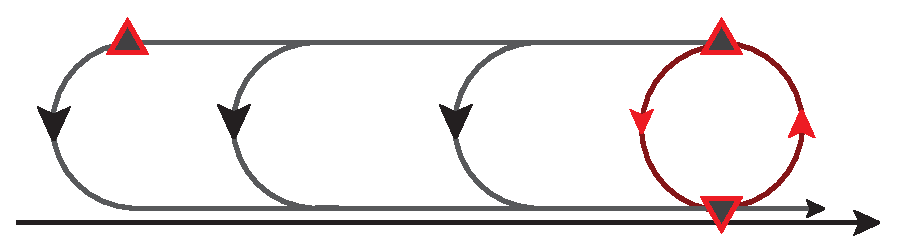
\includegraphics{StandardScheme.eps}
\caption{Стандартная схема}
\label{fig:StScheme}
\end{figure}


\begin{definition}{Поток - последовательность схем без циклов, оканчивающаяся схемой, которая содержит точку с флагом 'LAND'. Задаётся одной точкой --- начальной точкой какой-либо схемы.}
\end{definition}

%---------------------------------------------------------------------------------

\subsubsection{Файл с данными точек}

В первой строке указывается количество точек - число из $\mathbb{N}$

Далее перечисляются контрольные точки в соответствии следующему формату:

Имя начинается с буквы. Каждая точка в новой строке. Между элементами - пробел.

\bigskip

\begin{center}
Название $x$ $y$ $z$ $V_{min}$ $V_{max}$ флаг посадочной полосы
\end{center}

\bigskip

$x$, $y$, $z$ $\in \mathbb{R}$, где $x$ и $y$ - координаты в плоскости земли, а $z$ - вертикальная составляющая. Допускается ввод в метрах, километрах и морских милях.

$V_{min}$, $V_{max}$ $\in \mathbb{R}^+$, где $V_{min}$ - минимально допустимая скорость, а $V_{max}$ -- максимально допустимая скорость на данном контрольном пункте. Допускается ввод в метрах в секунду, километрах в час и морских милях в час.

флаг посадочной полосы -  'LAND' иначе пусто или ноль

Примеры:

\begin{itemize}
	\item  SS025 0 0 900 70 90
	\item  RW08L -21.5 18431.5 10 65 85 LAND
\end{itemize}

%---------------------------------------------------------------------------------

\subsubsection{Файл с данными об обычных и стандартных схемах}


В первой строке указывается количество схем - число из $\mathbb{N}$

Во второй строке указывается количество стандартных схем  - число из $\mathbb{N}$

Далее перечисляются все схемы в формате:

Название схемы - любой набор букв и цифр. Точки отделяются пробелами. После двоеточия начинать с начальной точки.

\bigskip

\begin{center}
Название схемы (точка начала схемы)(точки конца схемы) : название точек [спрямление] название точек
\end{center}

\bigskip

Формат для стандартных схем:

\bigskip

\begin{center}
Название стандартной схемы (точка начала стандартной схемы)(количество повторений стандартной схемы) : точка начала точка конца разворота точка конца обратного плеча
\end{center}

\bigskip

Некоторый "синтаксический сахар":

\begin{enumerate}
	\item В стандартной схеме можно опустить '(точка начала стандартной схемы)' и написать: Имя (количество повторений): T1 T2 T3
	\item Если схема состоит только из двух точек: 'NameTwoP (A)(B): A B', то можно опустить точки после двоеточия: 'NameTwoP (A)(B):'
\end{enumerate}

Примеры:
\begin{itemize}
	\item NameA (DIPOP)(EE500 KOLOS): Str(KOLOS) DIPOP EE500 /Str
	\item NameB (KOLOS)(BEKAR) : KOLOS VALET Str(RODEL) EE020 EE021 EE022 EE023 EE024 EE025 /Str RODEL BEKAR
	\item NameС (RODEL)(RW25R): RODEL BEKAR KVOTA EE252 EE253 RW25R
	\item NameStScheme (GALEB)(5): GALEB N1 N2
\end{itemize}

%---------------------------------------------------------------------------------

\subsubsection{Файл с данными о потоках}

В первой строчке количество потоков - число из $\mathbb{N}$

Далее каждый  поток в новой строке, согласно следующему правилу:

\begin{center}
Имя потока  Имя первой точки этого потока
\end{center}

Пример:
2\\
Flow1 DIPOP\\
Flow2 AKERA

\newpage

%==========================================================================================================

\subsection{Используемые структуры данных}

Из стандартной библиотеки шаблонов – STL были взяты в качестве массивов --- вектор и ассоциативный контейнер, также в алгоритмах используется стек. Для работы со строками используется класс string.

Реализованы следующие классы: координата, скорость и время с приватным конструктором и методами, позволяющими создавать экземпляры класса и возвращать значение в нужном виде. Перегрузка операторов $ '+~'$, $'-~'$, $'\ast~'$, $'/~'$, $'\ll~'$ в нужных случаях. Возведение в целую степень и извлечение квадратного корня для координаты.

\textbf{Основная информация хранится в структуре \textit{Zone}:}
\begin{enumerate}
	\item vector<vector<int$\gg$ graph\_of\_descendants;
	\item vector<CheckPoint> checkPoints;
	\item vector<Scheme> schemes;
	\item vector<Flow> flows;
	\item vector<StandardScheme> standardSchemes;
\end{enumerate}


Первое поле --- массив идентификаторов точек $\mapsto$ идентификаторы точек, которые можно достичь из данной. Второе массив структур контрольных точек. Третье --- массив структур схем. Четвёртое --- массив структур потоков. Пятое --- массив структур стандартных схем. Также Zone имеет различные методы для вывода информации на экран.

%---------------------------------------------------------------------------------

\textbf{Для хранения контрольных точек используется следующая структура --- \textit{CheckPoint}:}

\begin{enumerate}
	\item string name;
	\item Coordinate x = Coordinate::createMs(0);
	\item Coordinate y = Coordinate::createMs(0);
	\item Coordinate z = Coordinate::createMs(0);
	\item Velocity Vmin = Velocity::createVkm\_h(0);
	\item Velocity Vmax = Velocity::createVkm\_h(0);
	\item bool landing\_flag = false;
\end{enumerate}

Где первое поле --- это имя точки, второе, третье и четвёртые --- это координаты точки. Пятое и шестое --- скорости точки. И седьмое --- это флаг посадочной полосы.

%---------------------------------------------------------------------------------

\textbf{Для хранения схем --- \textit{Scheme}:}

\begin{enumerate}
	\item string name;
	\item int start;
	\item vector<int> end;
	\item vector<int> path;
	\item vector<int> straighteningFrom;
	\item vector<int> straighteningWhere
\end{enumerate}

Где первое поле --- это имя схемы, второе --- идентификатор точки, с которой начинается схема, третье --- конечные точки схемы. Четвёртое --- точки, которые образуют путь схемы, скелет. Пятое --- точки, с которых можно спрямляться и шестое --- точки, на которые допустимо спрямление.

%---------------------------------------------------------------------------------

\textbf{Для хранения потоков – \textit{Flow}:}

\begin{enumerate}
	\item string name;
	\item int start\_point;
	\item map<int, vector<int$\gg$ graph\_of\_descendants;
	\item map<int, vector<int$\gg$ graph\_of\_ancestors;
	\item vector<int> keys;
	\item map<int, vector<pair<Time, Time$\ggg$ times;
\end{enumerate}

Где первое поле --- имя потока, второе --- идентификатор точки начала потока. Третье --- отображение идентификатор точки $\mapsto$ идентификаторы точек, которые можно достичь из данной. Четвёртое --- отображение идентификатор точки $\mapsto$ идентификаторы точек, из которых можно достичь данной. Пятое --- массив ключей значений идентификаторов точек после топологической сортировки потока. И шестое --- идентификатор точки $\mapsto$ массив пар времён, где первый элемент пары --- минимально возможное время, за которое можно добраться до данной точки, а второй --- максимально возможное.

%---------------------------------------------------------------------------------

\textbf{Для хранения стандартных схем---\textit{StandardScheme}:}

\begin{enumerate}
	\item string name;
	\item int start;
	\item int second; 
	\item int third; 
	\item int repeat;
	\item Time Tmin = Time::createTsec(0);
	\item Time Tmax = Time::createTsec(0);
\end{enumerate}

Первое поле --- имя стандартной схемы. Второе --- идентификатор точки начала и конца стандартной схемы, третье --- идентификатор точки начала обратного плеча стандартной схемы, четвёртое --- идентификатор точки конца обратного плеча стандартной схемы. Пятое --- количество повторений стандартной схемы. Шестое и седьмое поля хранят минимальное и максимальное время прохождения данной схемы соответственно.

%---------------------------------------------------------------------------------

\textbf{Используемые отображения --- \textit{Maps}:}
\begin{enumerate}
	\item map<string, int> pointNameToID;
	\item map<int, int> startPointIDtoStSchemeID;
\end{enumerate}

Первое отображение --- название точки $\mapsto$ идентификатор точки. Второе --- отображение идентификатор точки начала стандартной схемы $\mapsto$ идентификатор стандартной схемы.

\newpage

%==============================================================================

\subsection{Описание алгоритмов работы программы}

\subsubsection{Чтение данных --- основная идея}

Чтение происходит в три этапа. Сначала считываются точки, потом схемы, затем потоки. Каждая читается с помощью регулярных выражений в соответствии с форматом.

Основная идея одинакова для всех трёх файлов. Процедура, соответствующая файлу, получает на вход путь к нему и массив структур, который требуется заполнить. Далее объявляется счётчик, который отвечает за движение по массиву. Затем делается попытка открыть файл. В случае успеха выводится сообщение об открытии файла, иначе выводится сообщение об ошибке, и программа останавливает свою работу. Если файл был открыт, то первым делом происходит считывание длины массива и проверка на не отрицательность этого числа. В случае, если полученная длина массива не положительна, то происходит остановка программы. Иначе длина массива становится равной полученному числу. Далее объявляется регулярное выражение для работы с данными из файла. 

Начинается основной цикл, в котором происходит заполнение массива. Файл читается построчно и построчно обрабатывается регулярным выражением до тех пор, пока не закончится файл. Первым делом делается проверка на успешность сопоставления регулярного выражения и строки. В случае неуспеха выводится сообщение о несоответствии формату. Также проверяется уникальность имён входных данных. Далее делается проверка на возможность доступа к текущей координате массива. В случае невозможности осуществить это программа заканчивает работу и предупреждает о нехватке выделенного места под элементы массива. Затем идёт заполнение, подробности которого можно найти ниже. И, наконец, после успешного наполнения массива, делается проверка и правка, чтобы действительная длина массива совпадала с декларируемой, если это не так то производится коррекция, после чего файл закрывается.


%---------------------------------------------------------------------------------


\subsubsection{Чтение точек}

Напомним содержимое структуры \textit{checkPoint}. Она состоит из семи полей:

\begin{enumerate}
	\item Имя точки
	\item Координата x
	\item Координата y
	\item Координата z
	\item Минимальная скорость Vmin
	\item Максимальная скорость Vmax
	\item Флаг посадочной полосы
\end{enumerate}

Согласно формату, в таком же порядке данные находятся в файле. Теперь рассмотрим регулярное выражение:

\begin{verbatim}
([a-z,A-Z]\w*)\s+([-+]?[0-9]*\.?[0-9]+)\s+([-+]?[0-9]*\.?[0-9]+)\s+
\end{verbatim}

\begin{verbatim}
([-+]?[0-9]*\.?[0-9]+)\s+([0-9]*\.?[0-9]+)\s+([0-9]*\.?[0-9]+)\s*(LAND|0)?\s*
\end{verbatim}

Первая группа захвата отвечает за имя точки. Согласно формату, имя начинается с буквы. Далее может быть любые комбинации букв и цифр.
Вторая, третья и четвёртая группы захвата одинаковые и предназначены для распознания действительного числа.
Пятая и шестая почти аналогичны предыдущим трём, но они захватывают не все действительные числа, а только неотрицательные.
И, наконец, седьмая ищет совпадение с флагом посадки LAND, нулём либо же отсутствует вовсе. Однако, одна и только одна точка с таким флагом должна быть. За корректность этого отвечает счётчик «k».

Далее происходит заполнение структуры \textit{CheckPoints} поэлементно, в зависимости от исходных данных. Поддерживается ввод в следующих единицах измерения: 
\begin{itemize}
	\item Координата в метрах, в километрах и в морских милях
	\item Скорость в метрах в секунду, километрах в час и морских милях в час
\end{itemize}

Флаг посадки по умолчанию $false$. $True$ присваивается, если седьмая группа захвата содержит LAND. И увеличивается счётчик «k». Если он превосходит единицу---программа останавливается и предупреждает об ошибке, что посадочных точек больше одной. Потом происходит заполнение отображения Имя точки $\mapsto$ идентификатор точки.
Затем происходит проверка корректности введённых скоростей, чтобы максимальная скорость не была меньше минимальной. И увеличивается счётчик «i».
Наконец, делается финальная проверка, что если <<k>> остался равен нулю, что означает отсутствие точки посадки, тогда программа завершает работу и предупреждает об ошибке.


%---------------------------------------------------------------------------------


\subsubsection{Чтение схем}

В файле со схемами лежит информация об обычных схемах и стандартных схемах. Начнём описание с обычных.

Напомним поля структуры \textit{scheme}:
\begin{enumerate}
	\item Имя схемы
	\item Идентификатор точки начала схемы
	\item Массив точек, которыми схема оканчивается
	\item Массив точек, составляющие основной путь схемы
	\item Массив точек, откуда можно спрямляться
	\item Массив точек, куда можно спрямляться
\end{enumerate}

Рассмотрим регулярное выражение и те части, которые относятся к обычной схеме:

\begin{verbatim}
(\w+)\s*(?:\((\w+)\))?\s*\(([\w\s]*|\d+)\)\s*:
\end{verbatim}

\begin{verbatim}
(?:\s*([\w\s]*)\s+(?:Str\(([\w\s]+)\)\s*([\w\s]+)\/Str)?\s*([\w\s]*)?)?
\end{verbatim}

Первая группа захвата --- это имя схемы. Представляет из себя любой набор букв и цифр.
Вторая группа --- это имя точки, с которой начинается схема.
Третья --- это имена точек, которой оканчивается схема.

Далее после двоеточия следует основное тело схемы. Четвертая группа — это точки схемы, предшествующие спрямлению. Если оно отсутствует, то эта группа представляет из себя путь. Однако, в связи с тем, что после этой группы обязательно должен быть хотя бы один пробел, и если после последней точки схемы пробела не будет, то эта точка не попадёт в эту группу захвата. Её нужно искать в седьмой.

Пятая группа --- это точки, на которые можно спрямляться с точек из шестой группы. Если спрямление в схеме отсутствует, то эти группы пустые. 
Седьмая группа --- это точки, идущие после спрямления. Или, если нет спрямления в схеме и нет пробела после последней точки, тогда тут находится та самая последняя точка.

Также для удобства записи схем состоящих из двух точек, было введено упрощение записи. Можно вводить только имя схемы, точку начала, точку конца и двоеточие. Что регулируется большой не захватывающей скобкой после двоеточия с вопросительным знаком на окончании.

Если спрямление присутствует, то путь состоит из четвёртой, шестой и седьмой групп захвата.

\large\textit{Заполнение}. \normalsize В общем случае первая группа сразу же присваивается в первое поле структуры. Второе поле – это результат отображения Имя точки $\mapsto$ идентификатор точки, где в качестве имени выступает вторая группа захвата.

Далее необходимо заполнить массив конечных точек. Для этого используется вспомогательная функция, которая получает строку на вход и массив, который требуется заполнить. Строка читается поэлементно, и с помощью отображения Имя точки $\mapsto$ идентификатор точки заполняет данный массив. В случае, если точки не оказалось среди \textit{checkPoints}, тогда выдаётся ошибка и программа заканчивает свою работу с предупреждением о том, что в такой-то строке такая-та точка не найдена среди контрольных точек.

Затем абсолютно аналогично заполняются поля пять и шесть. Теперь необходимо собрать путь схемы. Для этого используя ту же вспомогательную функцию с четвёртой группой и полем путь, мы собираем точки до спрямления. Затем записываем в путь все элементы из поля пять, и, наконец, используя вспомогательную функцию с седьмой группой и полем путь, мы собираем точки после спрямления.

Если четвёртая и пятая группы пустые, то это означает, что мы имеем дело со схемой, состоящей из двух точек. В этом случае, имя и точка начала схемы заполняются как в общем случае, но также нам известно, что массив конечных точек состоит из одного элемента, поэтому мы можем его сразу же записывать в массив конечных точек. И тогда путь, также легко определяется, как точка начала схемы плюс первый, он же и единственный, элемент массива конечных точек.

После чего увеличивается счётчик «i».

\bigskip

Теперь опишем работу со \textbf{\textit{стандартными схемами}}.

Напомним, что стандартной схемой называется схема типа «тромбон». Она определяется тремя точками и количеством повторений, что и отражено в полях структуры \textit{StandardScheme}:

\begin{enumerate}
	\item Имя схемы
	\item Идентификатор точки начала и конца стандартной схемы
	\item Идентификатор точки начала обратного плеча стандартной схемы
	\item Идентификатор точки конца обратного плеча стандартной схемы
	\item Количество повторений стандартной схемы
	\item Минимальное время, за которое можно пройти схему
	\item Максимальное время, за которое можно пройти схему
\end{enumerate}


Поля шесть, семь вычисляются в дальнейшем.

Рассмотрим регулярное выражение и те части, которые относятся к стандартной схеме:

\begin{verbatim}
(\w+)\s*(?:\((\w+)\))?\s*\(([\w\s]*|\d+)\)\s*:
\end{verbatim}

\begin{verbatim}
(?:\s*([\w\s]*)\s+(?:Str\(([\w\s]+)\)\s*([\w\s]+)\/Str)?\s*([\w\s]*)?)?
\end{verbatim}

Первая группа захвата --- это имя стандартной схемы. Так как начало и конец совпадают, то вторая группа захвата это второе поле структуры. Третья группа --- это количество повторений схемы.

В стандартной схеме нет спрямлений, поэтому пятая и шестая группы всегда пустые. Четвёртая и седьмая вместе дают все три точки. Поэтому с помощью вспомогательной функции из обычных схем, заполняем временный массив \textit{path}, аналогичный одноименному полю из обычных схем. И, затем, заполняем второе, третье и четвёртые поля структуры стандартной схемы как --- первый, второй и третий элемент массива \textit{path}. Если же длина этого массива получилась больше трёх, то программа завершает работу и выдаёт ошибку.

Далее заполняется отображение идентификатор точки начала стандартной схемы $\mapsto$ идентификатор стандартной схемы.

После чего увеличивается счётчик «k».

%---------------------------------------------------------------------------------


\subsubsection{Построение графа зоны}

Сначала заполняем поля времён у стандартных схем. Минимальное время --- пролёт по окружности с максимальной скоростью, а максимальное --- пролёт по всей схеме с минимальной скоростью.

Обозначим точки стандартной схемы $\nu_0 = (x_0, y_0, z_0),~ \nu_1 = (x_1, y_1, z_1),~ \nu_2 = (x_2, y_2, z_2)$
Вычислим радиус поворота, как половину от расстояния между $\nu_0$ и $\nu_1$:

$$
 R = \frac{1}{2} \ast \sqrt{(x_1 - x_0)^2 + (y_1 - y_0)^2 + (z_1 - z_0)^2}
$$

Длину плеча найдём, как расстояние между $\nu_1$ и $\nu_2$:

$$
S = \sqrt{(x_2 - x_1)^2 + (y_2 - y_1)^2 + (z_2 - z_1)^2}
$$

Тогда минимальное и максимальное времена выражаются следующим образом:


$$
T_{min} = \frac{2 \pi R}{v_{max}}, \hspace{3ex} T_{max} = \frac{2(S + \pi R)}{v_{min}}
$$


где $v_{max}$ и $v_{min}$ --- это максимально и минимально возможные скорости первой точки <<тромбона>>.

Граф зоны будем строить списками следующих. То есть соединяем ребрами данную вершину, со всеми вершинами, которые имеют связь с данной. Делать это будем следующим образом: идём по массиву схем, обрабатывая каждую схему в отдельности. На данном этапе нас интересует поле \textit{path}. Так как в нём лежат вершины в порядке прохождения самолётом схемы, то мы будем соединять текущую точку со следующей. Далее нужно соединить вершины, с которых возможно спрямление со всеми вершинами на которые это спрямление доступно. После чего переходить к другой схеме. Но есть нюанс. Если из предпоследней точки схемы можно спрямиться на конечную, то возникает проблема с добавлением этого ребра дважды --- первый раз как элемент пути, второй как элемент спрямления. Это необходимо учесть. 


%---------------------------------------------------------------------------------


\subsubsection{Построение потока}

Начальной точке потока выставляем $T_{min} = T_{max} = 0$. Теперь построим граф потока, как подграф графа зоны, также списками потомков. Для этого воспользуемся поиском в глубину. Заведём стек, на который будем складывать не посещённые вершины и массив меток, в котором будем отмечать посещённые вершины. Будем работать до тех пор, пока стек не опустеет. Сначала складываем на него точку начала потока. Используя граф зоны, соединяем эту точку со всеми сыновьями, и если сын ещё не посещён, то добавляем его на стек и ставим метку, что его посетили. В результате получим граф потока. После собираем граф потока, заданный списками предшественников, путём перебора графа, построенного списками потомков.



%---------------------------------------------------------------------------------


\subsubsection{Топологическая сортировка}

Данный ориентированный граф не имеет циклов, поэтому его можно топологически отсортировать, то есть сделать так, чтобы из вершин с меньшими номерами дуги шли в вершины с большими номерами. Для этой цели есть у потока поле \textit{keys}. Это массив, хранящий идентификатор в топологически отсортированном порядке $\mapsto$ идентификатор в исходном порядке. Сортировка проводится методом полустепеней захода. Заведём переменную \textit{number}, которая будет помогать отсортировывать вершины, инициализируем её нулём. Сначала сделаем размер массива ключей равным количеству вершин в потоке. Затем инициализируем отображение Точка $\mapsto$ полу степень захода следующим образом всем вершинам сопоставляется ноль. Заполняем его так: идя по спискам потомков, увеличиваем значение на единицу за каждого предка у вершины. Заводим стек и складываем на него все вершины с нулевой полустепенью захода. Пока стек не пуст, берём вершину со стека и на место number в массиве записываем идентификатор вершины. Увеличиваем \textit{number} на единицу. И для всех потомков данной вершины уменьшаем на единицу полустепень захода, и, если она стала равна нулю --- кладём этого потомка на стек. В результате получаем нужный массив.


%---------------------------------------------------------------------------------


\subsubsection{Объединение времён}

На вход дается массив пар действительных чисел. Необходимо объединить вложенные пары в одну, две пересекающиеся в одну. Будем делать с помощью отображения число$\mapsto$ действие. Для корректного сравнения действительных чисел реализованы два компаратора для проверки что одно число больше или меньше другого с точностью $\epsilon$, заданной в классе времени (по умолчанию $\epsilon = 10^{-4}$). Сначала проверим, что пары заданы корректно, то есть первый элемент меньше либо равен второго, иначе программа завершает работу и выдаёт сообщение об ошибке. Затем инициализируем нулевыми значениями отображение и заполняем его, если элемент стоит на первом месте в паре, тогда его значение увеличиваем на единицу, если на втором, то уменьшаем на единицу. Очистим массив времён. Заведём переменную, в которой будем считать сумму, инициализировав нулём. Вместе с тем, запомним первый элемент и назовём его начальным. Идём до конца ассоциативного массива, суммируя с накоплением значения отображения. Если в какой-то момент сумма стала равна нулю, то добавляем пару, состоящую из первого элемента, который мы запомнили, и текущего элемента. Проверяем, если мы не дошли до конца ассоциативного массива, то следующий элемент объявляем начальным и продолжаем цикл. В результате мы объединили вложенные и пересекающиеся интервалы, остались лишь не пересекающиеся.


%---------------------------------------------------------------------------------


\subsubsection{Расчёт времён}

Будем рассчитывать время для каждого потока по отдельности.

Так как поток топологически отсортирован, мы будем двигаться по возрастанию идентификатора вершин до тех пор, пока не дойдём до вершины с максимальным индексом, рассчитывая возможное время прибытия в следующие точки из данной. Сразу же выполним объединение времён, так как с прошлого шага мы получили набор интервалов, не обязательно не пересекающихся. 

Требует отдельного рассмотрения стандартная схема. Если в данная точка является началом стандартной схемы, у которой остались повторения, то нужно к текущим временным интервалам данной точки добавить интервалы, полученные прибавлением $T_{min}$ и $T_{max}$ из полей стандартной схемы к каждому из имеющихся интервалов данной точки, и уменьшить количество повторений этой стандартной схемы на единицу. 

Если же стандартной схемы нет или она исчерпала себя, то тогда для всех потомков время вычисляется как равнопеременное:

$$
T_{min} = \frac{2S}{v_{max}^0 + v_{max}^1}
$$
где $v_{max}^0$ --- это максимально допустимая скорость на текущей контрольной точке, а $v_{max}^1$ --- это максимально допустимая скорость на данном потомке текущей контрольной точке

$$
T_{max} = \frac{2S}{v_{min}^0 + v_{min}^1}
$$
где $v_{min}^0$ --- это минимально допустимая скорость на текущей контрольной точке, а $v_{min}^1$ --- это минимально допустимая скорость на данном потомке текущей контрольной точке

$S$ --- обычное Евклидово расстояние:

$$
S = \sqrt{(x_1 - x_0)^2 + (y_1 - y_0)^2 + (z_1 - z_0)^2)}
$$


После чего добавляем к каждому интервалу полученные $T_{min}$ и $T_{max}$, и этот новый интервал записываем в массив времён потомка. И увеличиваем счётчик на единицу. После выполнения цикла получаем набор временных интервалов для каждой точки из потока.

Выполняя данную процедуру для каждого из потоков получим набор временных интервалов для каждой точки.

После чего выводим на экран.

\newpage
%=======================================================================

\section{Численные расчёты}
\subsection{Простейшие случаи}

Рассмотрим работу процедуры в простейших случаях на данном примере:

\begin{figure}[h]
  \begin{center}
      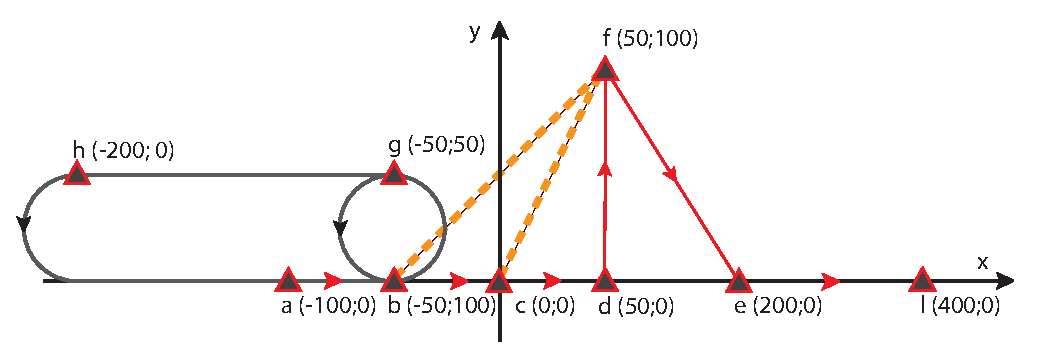
\includegraphics[scale=1]{Example.eps}
        \caption{Макетный пример}                                                                             
  \end{center}
\end{figure}

Пусть расстояние будет в метрах, а скорость в метрах в секунду.

\noindent Файл с данными точек:\\
9\\
a -100 0 0 5 10\\
b -50 0 0 5 10\\
c 0 0 0 5 10\\
d 50 0 0 5 10\\
e 200 0 0 4 6\\
f 50 100 0 4 8\\
g -50 50 0 5 10\\
h -200 50 0 5 10\\
r 400 0 0 2 5 LAND\\

\noindent Файл с данными схем:\\
3\\
1\\
Name1 (e)(r):\\
Name2 (a)(e): a Str(f) b c d /Str f e\\
NameSt1 (0): b g h\\

\noindent Файл с данными потоков:\\
3\\
Flow1 e\\
Flow2 a\\

\subsubsection{Движение по прямой}


Рассмотрим движение по прямой на примере первого потока:


$$
T_{min} = \frac{2S}{v_{max}^e + v_{max}^r} = \frac{2\cdot\sqrt{(400 - 200)^2}}{6 + 5} \approx 36.(36) ~sec
$$

$$
T_{max} = \frac{2S}{v_{min}^e + v_{min}^r} = \frac{2\cdot\sqrt{(400 - 200)^2}}{4 + 2} \approx 66.(66) ~sec
$$

И результат процедуры:

\noindent Flow1:\\
e $\rightarrow$ [0~sec, 0~sec]\\
r $\rightarrow$ [36.36~sec, 66.67~sec]


%---------------------------------------------------------------------------------

\subsubsection{Движение по вееру и прямым участкам}

Движение по вееру и прямым участкам рассмотрим на примере второго потока. Рассчитаем временной интервал для точки $f$:


\begin{eqnarray*}

T_{min} = \frac{2S_{a-b}}{v_{max}^b + v_{max}^a} + \frac{2S_{b-f}}{v_{max}^f + v_{max}^b}
= \frac{2\cdot\sqrt{(-50 + 100)^2}}{10 + 10} + \frac{2\cdot\sqrt{(50 + 50)^2 + (100-0)^2}}{8 + 10} \approx 20.71348 ~sec

\end{eqnarray*}

\begin{eqnarray*}

T_{max} = T_{max}^{a-b} + T_{max}^{b-c} + T_{max}^{c-d} + T_{max}^{d-f} = 
 \frac{2S_{a-b}}{v_{min}^b + v_{min}^a} + \frac{2S_{b-c}}{v_{min}^c + v_{min}^b} +
 \frac{2S_{c-d}}{v_{min}^d + v_{min}^c} + \frac{2S_{d-f}}{v_{min}^f + v_{min}^d} =
 \frac{2\cdot\sqrt{(-50 + 100)^2}}{5 + 5} + \frac{2\cdot\sqrt{(0 + 50)^2}}{5 + 5} +
 \frac{2\cdot\sqrt{(50 - 0)^2}}{5 + 5} + \frac{2\cdot\sqrt{(50 - 50)^2 + (100-0)^2}}{5 + 4}
 = 10 + 10 + 10 + 22.(2) = 52.(2) ~sec

\end{eqnarray*}


Результат процедуры:
Flow2:\\
a $\rightarrow$ [0 sec, 0 sec]\\
b $\rightarrow$ [5 sec, 10 sec]\\
c $\rightarrow$ [10 sec, 20 sec]\\
d $\rightarrow$ [15 sec, 30 sec]\\
f $\rightarrow$ [20.71 sec, 52.22 sec]\\
e $\rightarrow$ [46.47 sec, 97.29 sec]\\
r $\rightarrow$ [82.83 sec, 163.96 sec]\\


%---------------------------------------------------------------------------------

\subsubsection{Движение по вееру и прямым участкам со стандартной схемой}

Теперь изменим файл схем следующим образом --- добавим одно повторение к стандартной схеме:

\noindent 3\\
1\\
Name1 (e)(r):\\
Name2 (a)(e): a Str(f) b c d /Str f e\\
NameSt1 \underline{(1)}: b g h

И запустим поток с точки a:

\noindent 1\\
Flow1 a

Посчитаем время минимальной и максимальной задержки на <<тромбоне>>:

Вычислим радиус поворота, как половину от расстояния между b и g:

$$
 R = \frac{1}{2} \cdot \sqrt{(-50 + 50)^2 + (50 - 0)^2} = 25
$$

Длину плеча найдём, как расстояние между h и g:

$$
S = \sqrt{(-200 + 50)^2 + (50 - 50)^2} = 150
$$

$$
T_{min} = \frac{2 \pi R}{v_{max}^b} = \frac{2 \pi \cdot 25}{10} = 5\pi \approx 15.7
$$

$$
T_{max} = \frac{2(S + \pi R)}{v_{min}^b} = \frac{2(150 + \pi \cdot 25)}{5} = 60 + 10\pi \approx 91.4
$$

Результат процедуры:

\noindent Flow1:\\
a $\rightarrow$ [0 sec, 0 sec]\\
b $\rightarrow$ [5 sec, 10 sec] [20.71 sec, 101.42 sec]\\
c $\rightarrow$ [10 sec, 20 sec] [25.71 sec, 111.42 sec]\\
d $\rightarrow$ [15 sec, 30 sec] [30.71 sec, 121.42 sec]\\
f $\rightarrow$ [20.71 sec, 143.64 sec]\\
e $\rightarrow$ [46.47 sec, 188.71 sec]\\
r $\rightarrow$ [82.83 sec, 255.37 sec]\\


Как можно заметить, появился новый временной интервал соответствующий проходу по стандартной схеме.

\newpage

%======================================================================


\subsection{Расчёты для аэропорта <<Кольцово>>}

Рассмотрим работу программы на примере аэропорта Кольцово.

Общий вид зоны Кольцово представлен на рис.~\ref{KoltsAll}. Вид внутренней зоны представлен на рис.~ \ref{KoltsLand}

\begin{figure}[h]
  \begin{center}
      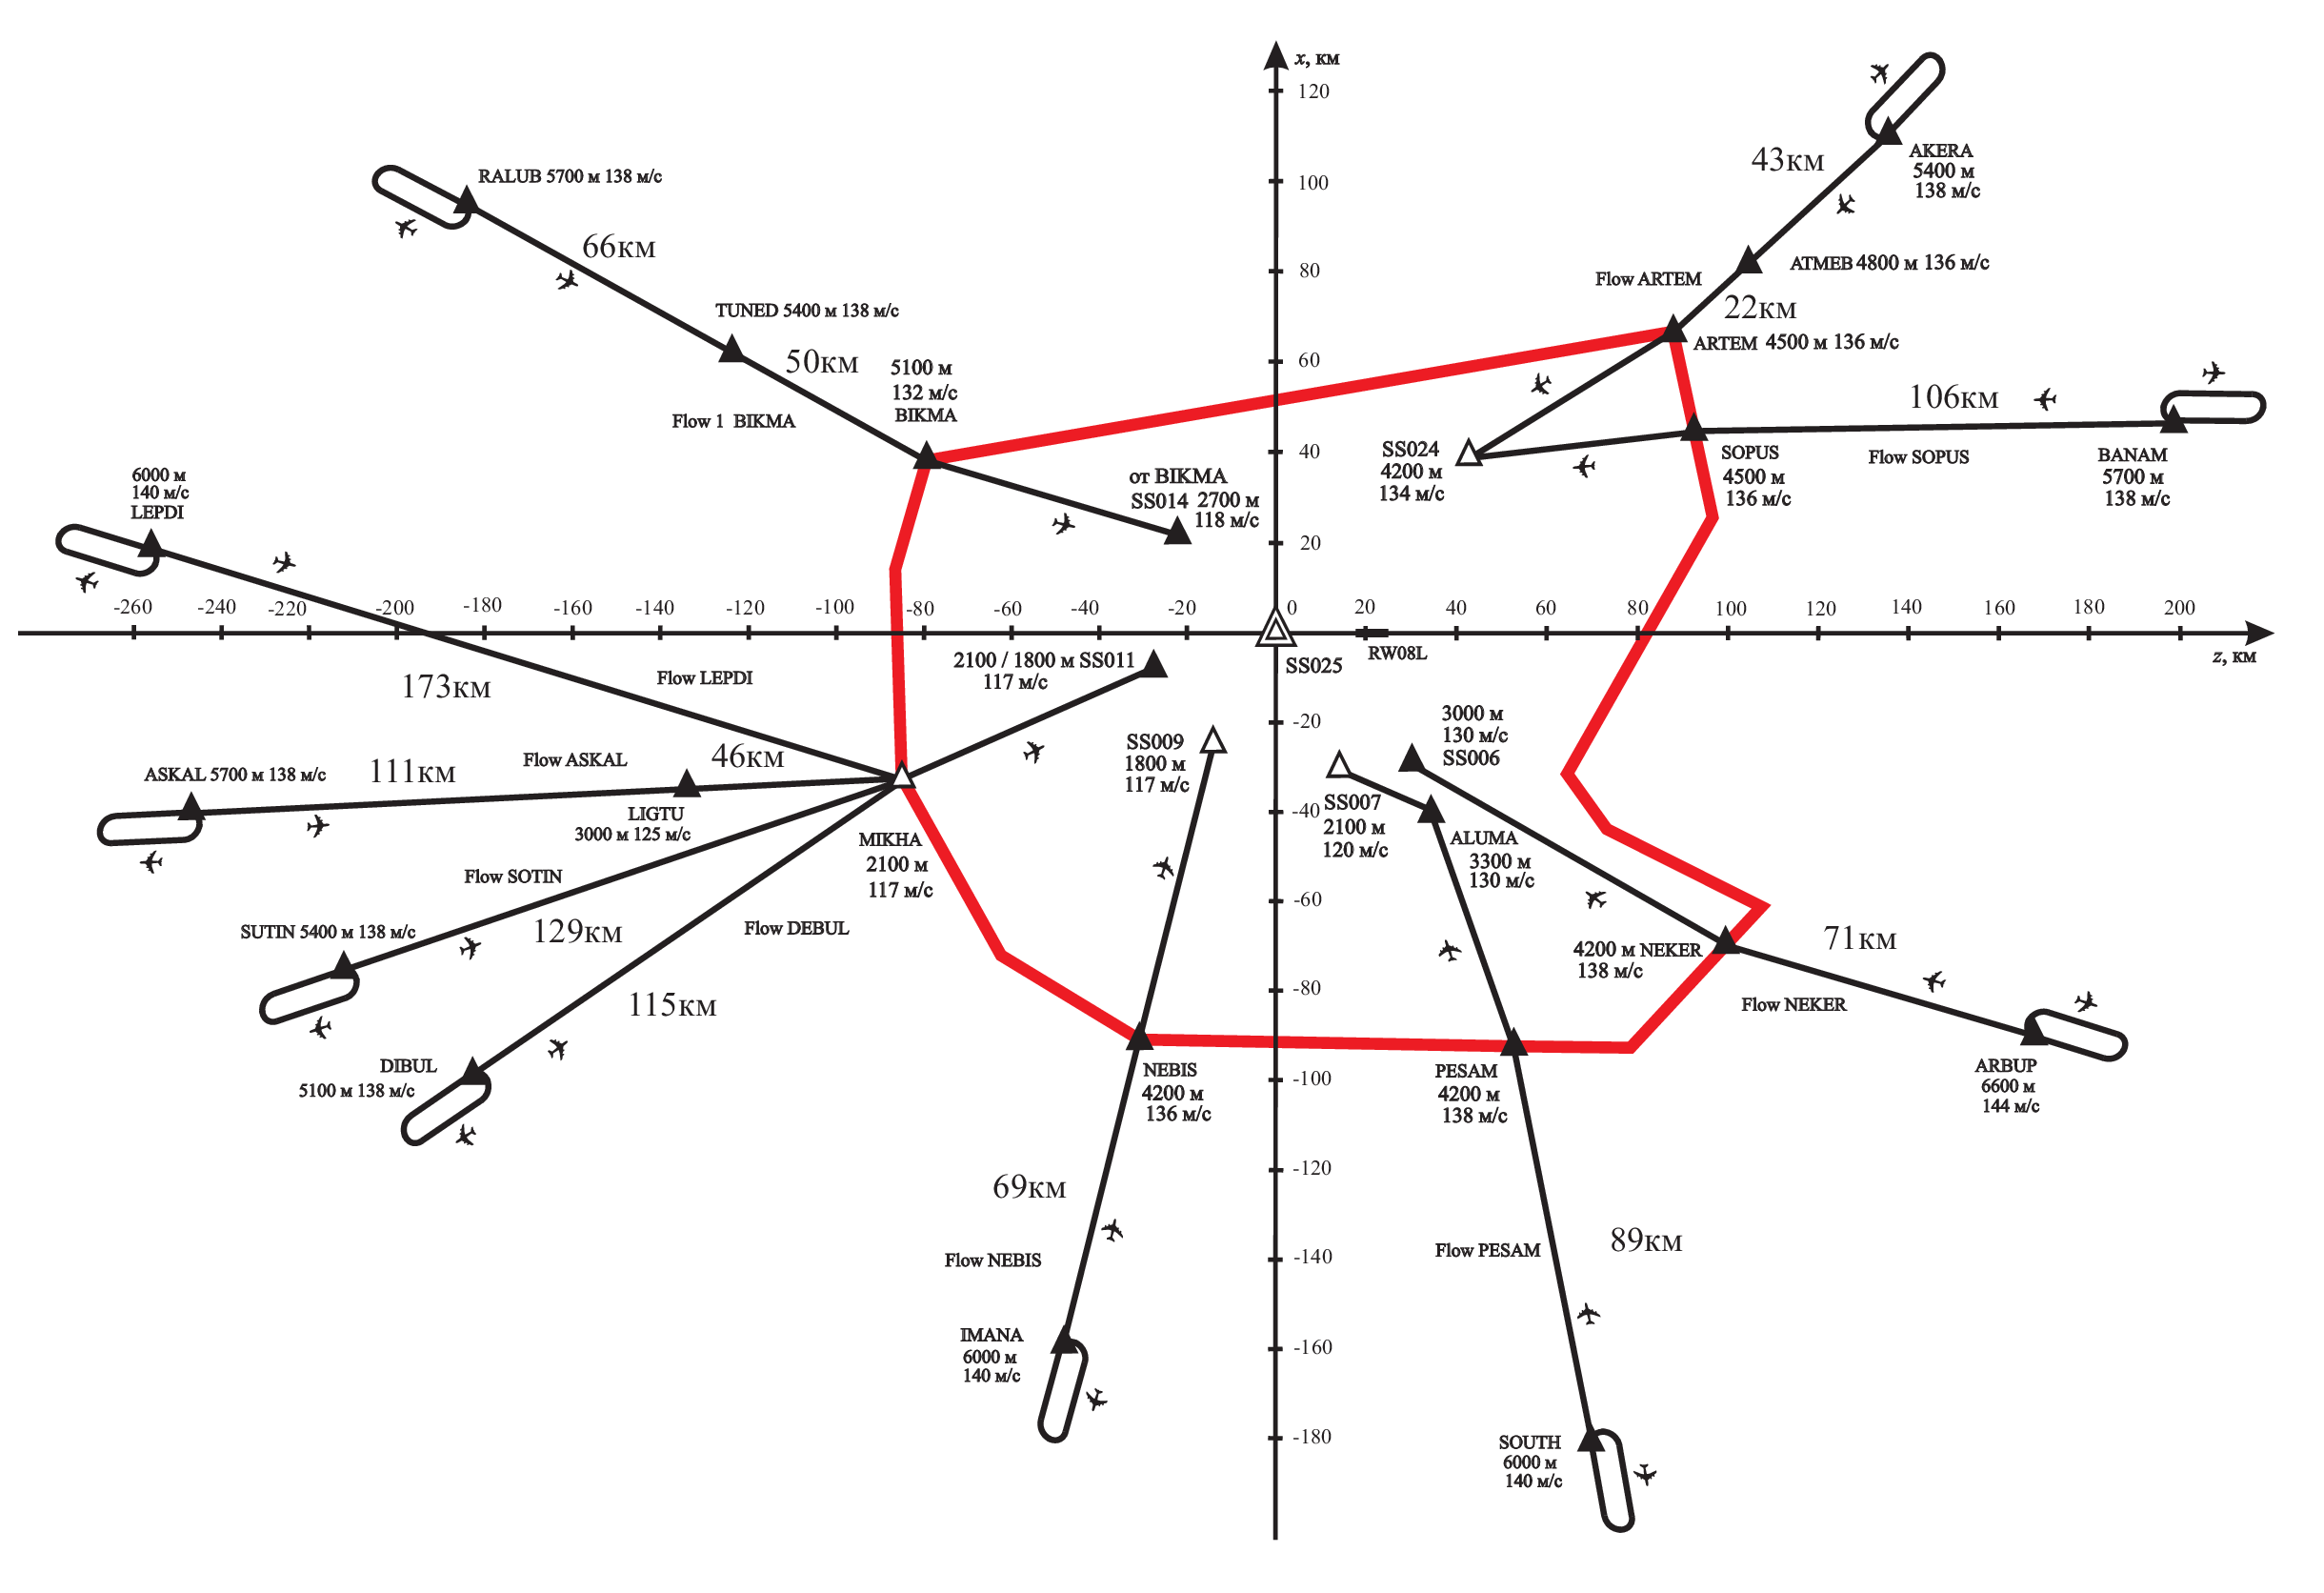
\includegraphics[scale=0.25]{Koltsovo01.png}
        \caption{Общий вид зоны Кольцово}                                                                             
    \label{KoltsAll}
  \end{center}
\end{figure}

\begin{figure}[h]
  \begin{center}
      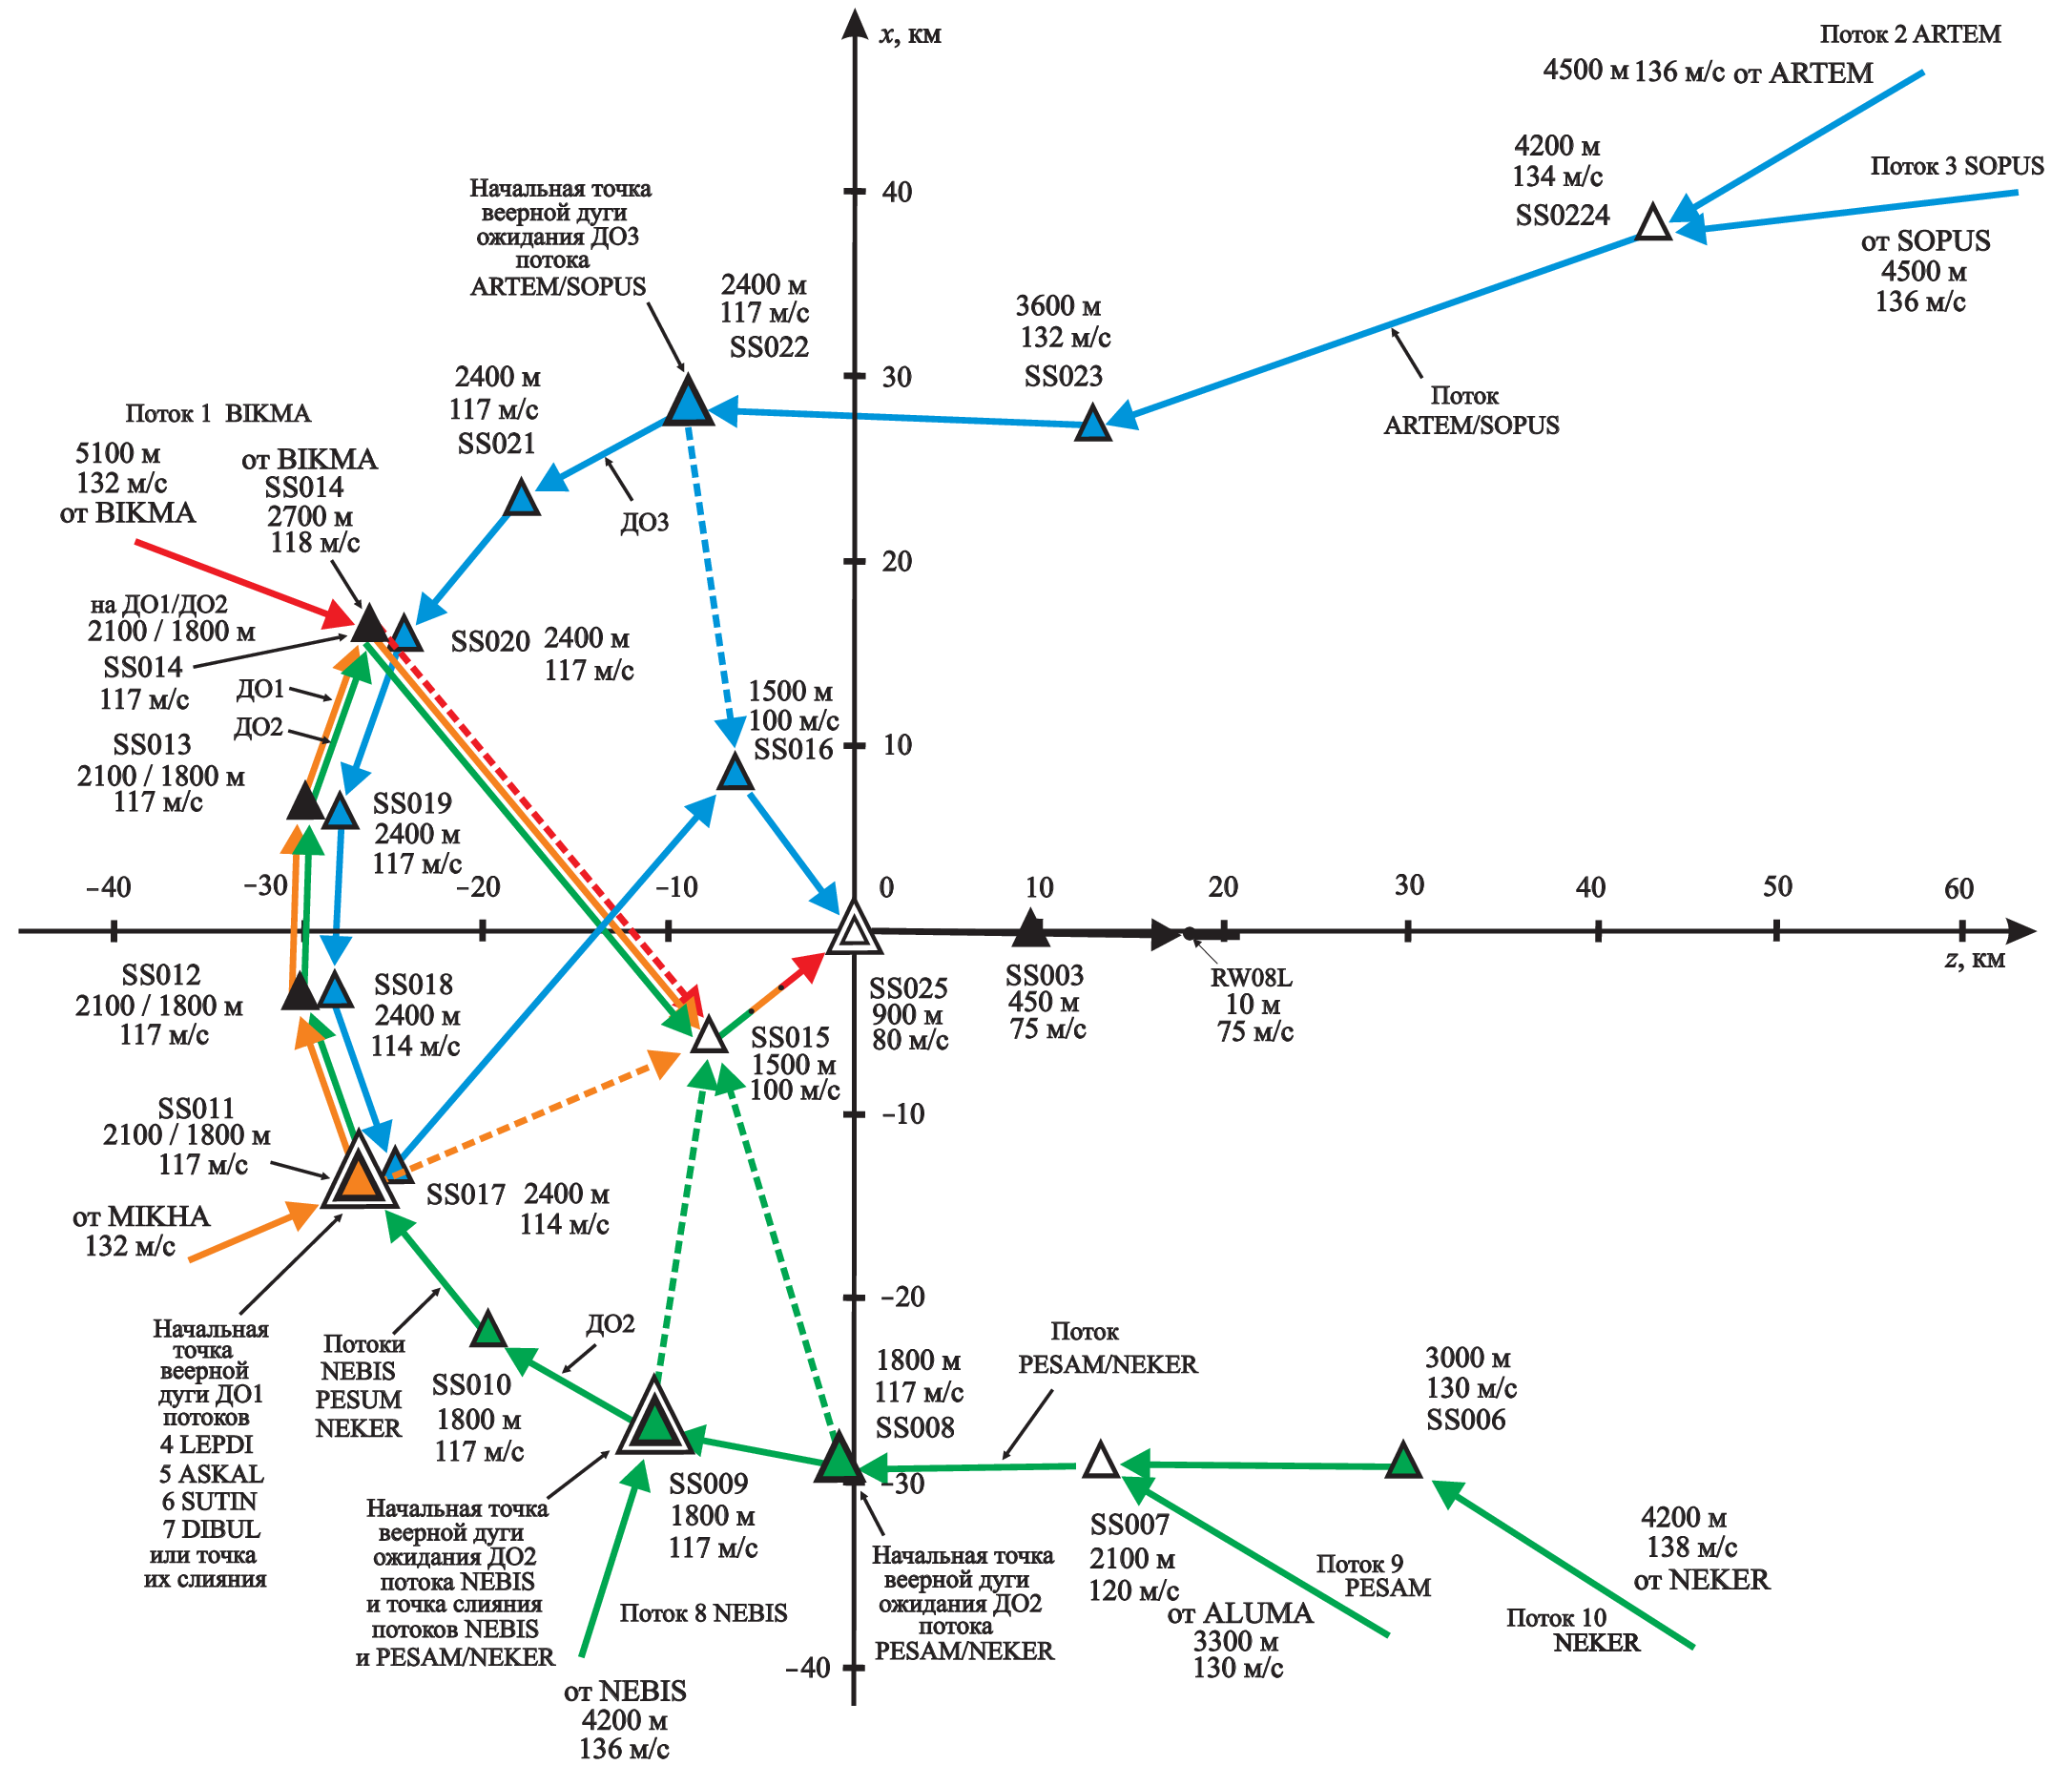
\includegraphics[scale=0.25]{Koltsovo02.png}
        \caption{Прибывающие потоки и веерные схемы их слияния.}                                                                             
    \label{KoltsLand} 
  \end{center}
\end{figure}

Рассмотрим поток BIKMA начинающийся в точке RALUB.

Результаты работы процедуры для потока BIKMA c нулём повторений стандартной схемы:

\noindent Flow1BIKMA:\\
RALUB $\rightarrow$ [0 sec, 0 sec]\\
TUNED $\rightarrow$ [474.52 sec, 548.67 sec]\\
BIKMA $\rightarrow$ [818.27 sec, 947.42 sec]\\
SS014 $\rightarrow$ [1240.52 sec, 1443.1 sec]\\
SS015 $\rightarrow$ [1482.57 sec, 1734.04 sec]\\
SS025 $\rightarrow$ [1578.33 sec, 1853.75 sec]\\
SS003 $\rightarrow$ [1684.27 sec, 1991.08 sec]\\
RW08L $\rightarrow$ [1792.31 sec, 2132.36 sec]\\


Результаты работы процедуры для потока BIKMA c однократным повторением стандартной схемы:

\noindent Flow1BIKMA:\\
RALUB $\rightarrow$ [0 sec, 0 sec] [389.33 sec, 992.17 sec]\\
TUNED $\rightarrow$ [474.52 sec, 548.67 sec] [863.86 sec, 1540.84 sec]\\
BIKMA $\rightarrow$ [818.27 sec, 947.42 sec] [1207.61 sec, 1939.58 sec]\\
SS014 $\rightarrow$ [1240.52 sec, 1443.1 sec] [1629.85 sec, 2435.26 sec]\\
SS015 $\rightarrow$ [1482.57 sec, 1734.04 sec] [1871.9 sec, 2726.21 sec]\\
SS025 $\rightarrow$ [1578.33 sec, 1853.75 sec] [1967.66 sec, 2845.91 sec]\\
SS003 $\rightarrow$ [1684.27 sec, 1991.08 sec] [2073.6 sec, 2983.24 sec]\\
RW08L $\rightarrow$ [1792.31 sec, 2132.36 sec] [2181.64 sec, 3124.52 sec]\\


Рассмотрим поток NEKER начинающийся в точке ARBUP.

Результаты работы процедуры для потока NEKER c нулём повторений стандартной схемы:

\noindent Flow10NEKER:\\
ARBUP $\rightarrow$ [0 sec, 0 sec]\\
NEKER $\rightarrow$ [463.24 sec, 533.96 sec]\\
SS006 $\rightarrow$ [1015.68 sec, 1175.5 sec]\\
SS007 $\rightarrow$ [1140.14 sec, 1321.61 sec]\\
SS008 $\rightarrow$ [1249.54 sec, 1451.18 sec]\\
SS009 $\rightarrow$ [1331.5 sec, 1548.45 sec]\\
SS010 $\rightarrow$ [1413.66 sec, 1645.98 sec]\\
SS011a $\rightarrow$ [1496.1 sec, 1743.82 sec]\\
SS012a $\rightarrow$ [1578.68 sec, 1841.84 sec]\\
SS013a $\rightarrow$ [1661.3 sec, 1939.91 sec]\\
SS014aaa $\rightarrow$ [1743.95 sec, 2038 sec]\\
SS015 $\rightarrow$ [1455.79 sec, 2330.19 sec]\\
SS025 $\rightarrow$ [1551.56 sec, 2449.89 sec]\\
SS003 $\rightarrow$ [1657.5 sec, 2587.22 sec]\\
RW08L $\rightarrow$ [1765.54 sec, 2728.5 sec]\\



Результаты работы процедуры для потока NEKKER c однократным повторением стандартной схемы в точке ARBUP:

\noindent Flow10NEKER:\\
ARBUP $\rightarrow$ [0 sec, 0 sec] [234.91 sec, 925.33 sec]\\
NEKER $\rightarrow$ [463.24 sec, 533.96 sec] [698.15 sec, 1459.29 sec]\\
SS006 $\rightarrow$ [1015.68 sec, 1175.5 sec] [1250.59 sec, 2100.83 sec]\\
SS007 $\rightarrow$ [1140.14 sec, 1321.61 sec] [1375.04 sec, 2246.93 sec]\\
SS008 $\rightarrow$ [1249.54 sec, 1451.18 sec] [1484.45 sec, 2376.51 sec]\\
SS009 $\rightarrow$ [1331.5 sec, 1548.45 sec] [1566.4 sec, 2473.78 sec]\\
SS010 $\rightarrow$ [1413.66 sec, 1645.98 sec] [1648.57 sec, 2571.31 sec]\\
SS011a $\rightarrow$ [1496.1 sec, 2669.15 sec]\\
SS012a $\rightarrow$ [1578.68 sec, 2767.16 sec]\\
SS013a $\rightarrow$ [1661.3 sec, 2865.24 sec]\\
SS014aaa $\rightarrow$ [1743.95 sec, 2963.33 sec]\\
SS015 $\rightarrow$ [1455.79 sec, 3255.51 sec]\\
SS025 $\rightarrow$ [1551.56 sec, 3375.21 sec]\\
SS003 $\rightarrow$ [1657.5 sec, 3512.54 sec]\\
RW08L $\rightarrow$ [1765.54 sec, 3653.83 sec]\\

\newpage
%=======================================================================

\section*{Заключение}
\addcontentsline{toc}{section}{Заключение}

В результате работы была решена поставленная задача о вычислении временных интервалов прибытия воздушного судна на контрольные точки. Процесс работы состоял в изучении задачи, выборе структур данных и алгоритмов. Реализации на языке C{}\verb!++! 14-го стандарта. В качестве примера была рассмотрена схема аэропорта <<Кольцово>> в городе Екатеринбурге.

\newpage
%=======================================================================


\begin{thebibliography}{9}
\addcontentsline{toc}{section}{Список литературы}

\bibitem{bib:grafAndMatr} Асанов, М. О. Дискретная математика: графы, матроиды, алгоритмы : учебное пособие / М. О. Асанов, В. А. Баранский, В. В. Расин. — 2-е изд. испр. и доп. — Санкт-Петербург : Лань, 2010. — 368 с. — ISBN 978-5-8114-1068-2. 

\bibitem{bib:Report:2019-07} Спиридонов А.А. Кумков С.С. Разработка и исследование формализаций задачи бесконфликтного слияния потоков воздушных судов. Отчёт о научно-экспериментальной работе «Алгоритмы и программное обеспечение обработки информации в АС УВД» по Договору №29-19У. (Этап~1). Том~3, июнь 2019 г., 25~стр.
 
\bibitem{bib:TblSherem} Проект структуры воздушного пространства МУДР. Стандартные маршруты прибытия на аэродром Шереметьево. Версия 03 ПСВП МУДР 8.5.1 (таблицы). ГосНИИГА, Москва, 2016.

\bibitem{bib:SchmSherem} Проект структуры воздушного пространства МУДР. Схемы захода на посадку на аэродром Шереметьево. Версия 03 ПСПВ. Стандартные маршруты прибытия на аэродром Шереметьево. Версия 04 ПСВП МУДР 8.5.1 (схемы). ГосНИИГА, Москва, 2016.

\bibitem{bib:EURO} Point Merge Integration of Arrival Flows Enabling Extensive RNAV Application and Continuous Descent. Operation Services and Environment Definition. Report, July 2010. Eurocontrol Experimental Center, Bretigny-sur-Orge.\\
\texttt{http://www.eurocontrol.int/eec/gallery/content/public..}

\bibitem{bib:NASA} Air Traffic Management Technology Demonstration--1 (ATD--1). NASA Report FS-2011-10-01-ARC. 2011.

\bibitem{bib:NITA} Пятко С.Г., Красов А.И. и др. Автоматизированные системы управления воздушным движением. Новые информационные технологии в авиации. Санкт-Петербург; Изд. Политехника, 2004.

\bibitem{bib:KorolevEN} Королев Е. Н. Технологии работы диспетчеров управления воздушным движением.~-— Москва: Воздушный транспорт, 2000.

\bibitem{bib:GOST} ГОСТ 20058-80. Динамика летательных аппаратов в атмосфере. Термины, определения и обозначения.~---Москва: Госстандарт, 1980.


\end{thebibliography}


\end{document}
